% 71. hodina. Zdroj: učebnice/02_Funkce_a_rovnice/
% Funkce_s_absolutni_hodnotou/Lineární funkce s abs.tex,
% oddíl Funkce s více absolutními hodnotami; Realisticky.cz 020404–020405.
% Výklad a příklady autorsky upravené pro 45 minut a návaznost na hodinu 70.
\documentclass[11pt,a4paper]{article}
\input{../../sablony/pripravy/priprava.sty}
\usepackage{tikz}
\nastavPripravu{1. ročník}{Funkce}{71}{Grafy se dvěma absolutními hodnotami}
\begin{document}
\blok{Návaznost a hlavní myšlenka}
V minulé hodině měl předpis jednu absolutní hodnotu, a proto se graf rozdělil na dvě lineární větve. \textbf{Dvě absolutní hodnoty} mohou měnit znaménko na dvou různých místech: osu pak rozdělíme na \textbf{tři části}. V každé části odstraníme absolutní hodnoty podle znaménka výrazu \emph{uvnitř} a získáme obyčejnou lineární funkci.
\blok{Společný vzor: $f(x)=|x-4|+|x+4|$}
\begin{prikladReseniBox}[title={Příklad 1}]
Najděte nulové body obou výrazů v absolutních hodnotách a určete části osy, na kterých mají stálé znaménko.
\tcblower
$x-4=0\Rightarrow x=4$, $x+4=0\Rightarrow x=-4$. Získáme intervaly $(-\infty;-4)$, $\langle-4;4\rangle$ a $(4;+\infty)$. V krajních bodech je odpovídající absolutní hodnota nulová, proto můžeme tyto body přiřadit kterémukoliv sousednímu předpisu; pro přehlednost je zahrneme do prostřední části.
\end{prikladReseniBox}
\begin{center}
\small
\renewcommand{\arraystretch}{1.18}
\begin{tabular}{@{}lccc@{}}
\toprule
& $x<-4$ & $-4\le x\le4$ & $x>4$\\ \midrule
$x-4$ & $-$ & $-\ (\text{nebo }0)$ & $+$\\
$x+4$ & $-$ & $+\ (\text{nebo }0)$ & $+$\\
$|x-4|$ & $4-x$ & $4-x$ & $x-4$\\
$|x+4|$ & $-x-4$ & $x+4$ & $x+4$\\ \midrule
$f(x)$ & $-2x$ & $8$ & $2x$\\ \bottomrule
\end{tabular}
\end{center}
\begin{prikladReseniBox}[title={Příklad 2}]
Z předchozí tabulky zapište funkci po částech, sestrojte její graf a určete $D(f),H(f)$, minimum a monotónní části.
\tcblower
\[
f(x)=\begin{cases}-2x,&x<-4,\\8,&-4\le x\le4,\\2x,&x>4.\end{cases}
\]
Graf tvoří dvě šikmé polopřímky a vodorovná úsečka mezi body $[-4;8]$ a $[4;8]$. Platí $D(f)=\mathbb R$, $H(f)=\langle8;+\infty)$. Minimum je $8$ a nastává \textbf{pro všechna} $x\in\langle-4;4\rangle$ (nikoliv jen v jednom bodě). Funkce klesá na $(-\infty;-4\rangle$, je konstantní na $\langle-4;4\rangle$ a roste na $\langle4;+\infty)$. Je sudá, ale není prostá.
\end{prikladReseniBox}
\begin{center}
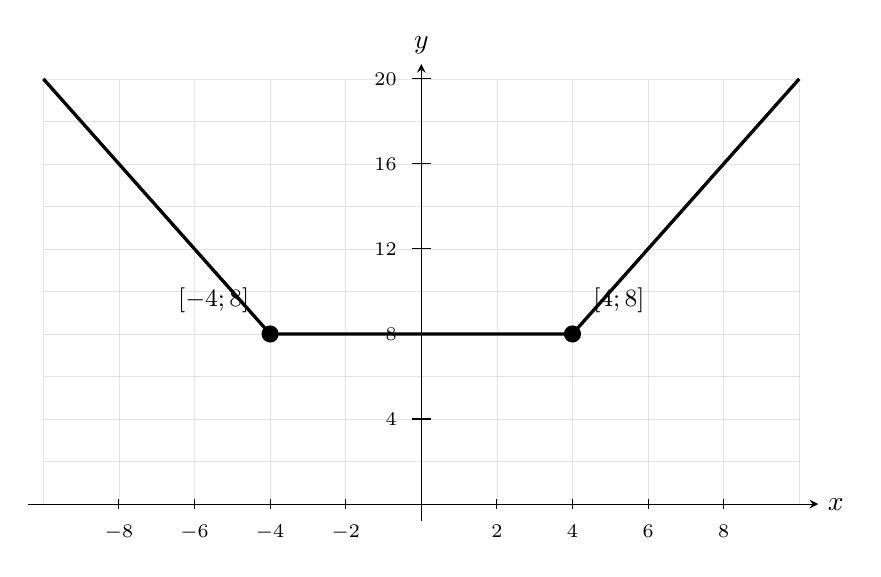
\begin{tikzpicture}[x=.48cm,y=.27cm,>=stealth]
\draw[step=2,gray!22,very thin] (-10,0) grid (10,20);
\draw[->] (-10.4,0)--(10.5,0) node[right] {$x$};
\draw[->] (0,-.8)--(0,20.7) node[above] {$y$};
\foreach \x in {-8,-6,-4,-2,2,4,6,8} {\draw (\x,.25)--(\x,-.25) node[below=2pt] {\scriptsize $\x$};}
\foreach \y in {4,8,12,16,20} {\draw (.25,\y)--(-.25,\y) node[left=2pt] {\scriptsize $\y$};}
\draw[very thick] (-10,20)--(-4,8)--(4,8)--(10,20);
\fill (-4,8) circle (3.1pt) node[above left=4pt] {\small $[-4;8]$};
\fill (4,8) circle (3.1pt) node[above right=4pt] {\small $[4;8]$};
\end{tikzpicture}
\end{center}
\poznamka{Kontrolní otázka: proč prostřední část není další véčko? Na $\langle-4;4\rangle$ se členy $-x$ a $x$ přesně vyruší. Zkontroluj výsledek dosazením $x=-5,0,5$: $10,8,10$. Matematický zápis hranic intervalů musí být konzistentní.}
\blok{Návod pro libovolné dvě absolutní hodnoty}
\begin{enumerate}[label=\arabic*.]
\item Polož \textbf{každý výraz uvnitř modulu} roven nule.
\item Seřaď získané hodnoty od nejmenší a rozděl podle nich osu.
\item V každé oblasti urči znaménka \emph{uvnitř} obou modulů a správně je odstraň.
\item Uprav na lineární předpis, nakresli jeho \emph{příslušnou část}; ověř shodu hodnot v bodech přechodu.
\end{enumerate}
\blok{Druhý společný příklad}
\begin{prikladReseniBox}[title={Příklad 3}]
Sestrojte $g(x)=|x-2|+|x+1|$. Určete body změny, předpis po částech a minimum.
\tcblower
Body změny jsou $x=-1$ a $x=2$. Pro jednotlivé části:
\[
g(x)=\begin{cases}1-2x,&x<-1,\\3,&-1\le x\le2,\\2x-1,&x>2.\end{cases}
\]
Krajní body vodorovné úsečky jsou $[-1;3]$ a $[2;3]$. Minimum $3$ nastává pro všechna $x\in\langle-1;2\rangle$ a $H(g)=\langle3;+\infty)$.
\end{prikladReseniBox}
\blok{Samostatné procvičování}
\begin{zadaniReseniBox}[title={Samostatná práce 1}]
\begin{enumerate}[label=\alph*)]
\item Sestrojte $p(x)=|x+2|+|x-2|$. Určete $H(p)$ a množinu argumentů, v nichž má minimum.
\item U $q(x)=|x-2|-|x+1|$ sestavte předpis po částech. Určete $H(q)$.
\end{enumerate}
\tcblower
\begin{enumerate}[label=\alph*)]
\item $p(x)=\begin{cases}-2x,&x<-2,\\4,&-2\le x\le2,\\2x,&x>2.\end{cases}$ Minimum $4$ nastává na $\langle-2;2\rangle$, $H(p)=\langle4;+\infty)$.
\item $q(x)=\begin{cases}3,&x<-1,\\1-2x,&-1\le x\le2,\\-3,&x>2.\end{cases}$ Výstupy jsou všechna čísla od $-3$ do $3$: $H(q)=\langle-3;3\rangle$. Kontrola v hranicích: $q(-1)=3$, $q(2)=-3$.
\end{enumerate}
\end{zadaniReseniBox}
\blok{Volitelná rezerva}
\begin{zadaniReseniBox}[title={Rozšíření 1}]
Sestrojte $r(x)=|2x-2|+|x+2|$. Určete body změny a nejmenší hodnotu.
\tcblower
Body změny: $x=-2$ a $x=1$.
\[
r(x)=\begin{cases}-3x,&x<-2,\\4-x,&-2\le x\le1,\\3x,&x>1.\end{cases}
\]
Minimum $3$ nastává v $x=1$; $H(r)=\langle3;+\infty)$.
\end{zadaniReseniBox}
\blok{Domácí úkol}
\begin{zadaniReseniBox}[title={Domácí úkol}]
\begin{enumerate}[label=\alph*)]
\item Pro $f(x)=|x-3|+|x+1|-2$ určete předpis po částech, minimum a $H(f)$.
\item Sestrojte $g(x)=|x-1|+|x+3|$. Určete interval konstantnosti a $D(g),H(g)$.
\item Vysvětlete, proč $h(x)=|x-4|+|x+4|$ není prostá a na kterých intervalech je konstantní.
\end{enumerate}
\tcblower
\begin{enumerate}[label=\alph*)]
\item $f(x)=\begin{cases}-2x,&x<-1,\\2,&-1\le x\le3,\\2x-4,&x>3.\end{cases}$ Minimum $2$ na $\langle-1;3\rangle$ a $H(f)=\langle2;+\infty)$. 
\item $g(x)=\begin{cases}-2x-2,&x<-3,\\4,&-3\le x\le1,\\2x+2,&x>1.\end{cases}$ Je konstantní na $\langle-3;1\rangle$, $D(g)=\mathbb R$ a $H(g)=\langle4;+\infty)$.
\item Např. $h(-5)=10=h(5)$, přesto $-5\ne5$; konstantní na $\langle-4;4\rangle$.
\end{enumerate}
\end{zadaniReseniBox}
\poznamka{Jádro 45 min: návaznost 4, ústřední příklad včetně tabulky a grafu 20, druhý příklad společně 8, samostatný pokus s kontrolou 11, zadání domácí práce 2 min. Záporné znaménko před absolutní hodnotou a nestejná směrnice jsou nadstavba, nikoli povinná nová látka. Připravit ke kreslení souřadnicovou síť.}
\end{document}
